%! TEX root = ../../master.tex
\lecture[]{Sa 18 Sep 2021}{test}

\begin{theorem}\label{thm:überlagerung-von-cw-komplex-ist-überlagerung}
    Jede Überlagerung eines CW-Komplexes ist ein CW-Komplex. Insbesondere ist eine Überlagerung eines Graphen wieder ein Graph.
\end{theorem}
%\begin{rproof}{thm:überlagerung-von-cw-komplex-ist-überlagerung}[skizziert]
%    Sei $X$ ein CW-Komplex und  $p\colon E \to  X$ eine Überlagerung.
%\[
%    \begin{tikzcd}
%        & E \ar{d}{p} \\
%        \underbrace{c_{α}}_{\text{zusammenziehbar}} \ar[dashed]{ur}\ar{r} & X 
%    \end{tikzcd}
%\]
%Da die $k$-Zellen von  $X$ zusammenziehbar sind, existiert jeweils eine Hebung  $\tilde{φ}_α\colon c_α \to  E$. Die Hebung solch einer $k$-Zelle von $X$ ist eine $k$-Zelle, also ergibt sich eine CW-Komplex Struktur auf $E$.
%\end{rproof}

\begin{example}
    Betrachte die Überlagerung $S^1 \to  S^1$ gegeben durch $z \mapsto z^2$, d.h.
\[
    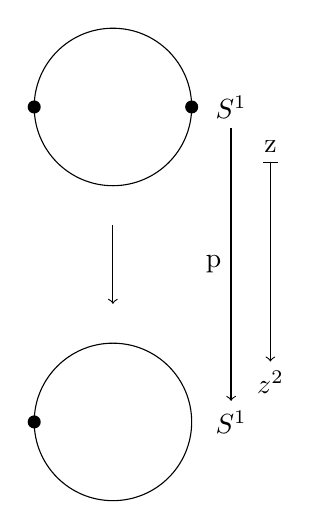
\begin{tikzpicture}
        \draw (0,2) circle (1);
        \node[fill, circle, scale=0.5] at (1,2) {};
        \node[fill, circle, scale=0.5] at (-1,2) {};
        \draw (0,-2) circle (1);
        \node[fill, circle, scale=0.5] at (-1,-2) {};
        \draw[->] (0,0.5) -- (0,-0.5);
        \node (A) at (1.5,2) {$S^1$};
        \node (A1) at (2,1.5) {z};
        \node (B) at (1.5, -2) {$S^1$};
        \node (B1) at (2,-1.5) {$z^2$};
        \draw[->] (A.south) -- (B.north) node[anchor=east, midway] {p};
        \draw[|->] (A1.south) -- (B1.north);
    \end{tikzpicture}
    \qquad
    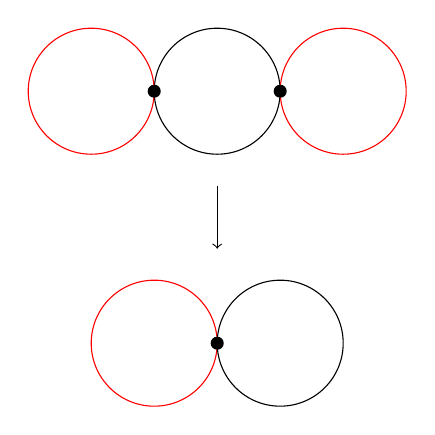
\begin{tikzpicture}[scale=0.8]
        \draw (0,2) circle (1);
        \draw[red] (-2,2) circle (1);
        \draw[red] (2,2) circle (1);
        \node[fill, circle, scale=0.5] at (1,2) {};
        \node[fill, circle, scale=0.5] at (-1,2) {};
        \draw[red] (-1,-2) circle (1);
        \draw (1,-2) circle (1);
        \node[fill, circle, scale=0.5] at (0,-2) {};
        \draw[->] (0,0.5) -- (0,-0.5);
    \end{tikzpicture}
\]
Wir sehen nun, dass die beiden Hebungen der 1-Zelle von $S^1$ nun die beiden 1-Zellen von  $E$ sind. Betrachte nun als zweites Beispiel die rechte Überlagerungen, wobei beide roten Zellen auf die rote abbilden, und die schwarze Zelle mittels $z \mapsto z^2$ abbildet. Dann sehen wir ebenfalls wieder jeweils die beiden Hebungen der beiden Zellen als vier 1-Zellen des Überlagerungsraums.
\end{example}

\begin{example}
    Betrachte die Überlagerung $\R \to  S^1$ durch $z \mapsto e^{iz}$, dann sind zunächst die Hebungen von $S^1$ jeweils die Intervalle  $[n,n+1]$ in  $\R$. Wir erweitern nun zu $S_1 \twedge S^1$ und hängen die entsprechenden Schleifen an den Überlagerungsraum an. Dann ergibt sich folgendes Bild:
    \missingfigure{Überlagerung von $S^1 \twedge S^1$}
\end{example}

\begin{example}[Universelle Überlagerung von $S^1 \twedge S^1$]
    Wir betrachten nun noch die universelle Überlagerung von $S^1 \twedge S^1$, die durch den folgenden Cayley-Graphen von $F_2$ gegeben ist. Man beachte, dass die 'Rekursion' im Bild zwar unendlich fortgesetzt wird, es sich allerdings dennoch nicht um die Teilraumtopologie handelt, die Punkte 'konvergieren' nicht. Wir bilden nun die horizontalen Segmente, die dem Erzeuger $a$ entsprechen, auf den roten Kreis ab, die vertikalen auf den blauen.

\begin{tikzpicture}
    \node (label) at (0,0) {
    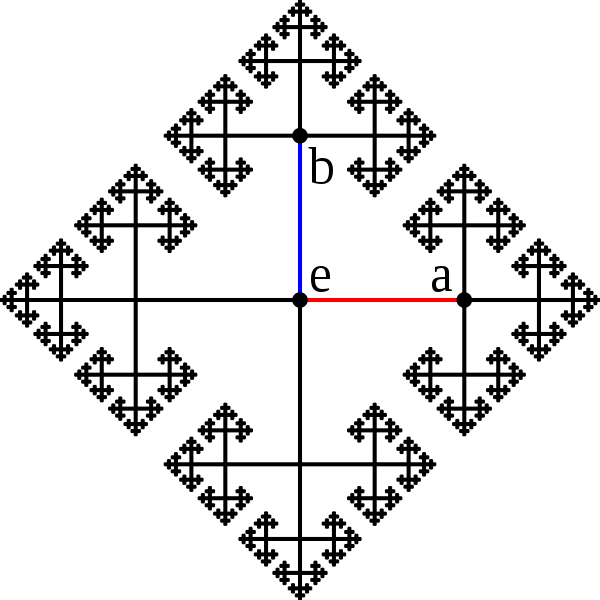
\includegraphics[scale=0.25]{figures/600px-Cayley_graph_of_F2.svg.png}
};
    \draw[red] (5,0) circle (1);
    \draw[blue] (7,0) circle (1);
    \node[scale=0.5, fill, circle] at (6,0) {};
    \draw[->] (label.east) -- (3.5, 0);
    \node at (label.south) {\tiny Bild von \cite{img:cayley-graph-f2}};
\end{tikzpicture}
\end{example}

\begin{corollary}\label{cor:untergruppe-von-freier-gruppe-ist-frei}
    Jede Untergruppe einer freien Gruppe ist frei.
\end{corollary}
\begin{proof*}
    Wir können die freie Gruppe durch einen Graphen mit entsprechend vielen Schleifen darstellen. Untergruppen entsprechen nun aber Überlagerungen. Solch eine Überlagerung ist aber  wieder ein Graph und hat damit eine freie Fundamentalgruppe. Also ist die Untergruppe frei!
\end{proof*}

\begin{theorem}[2-dimensionale Komplexe]
    Sei $X$ ein wegzusammenhängender Raum. Gegebn eine Familie von Abbildungen
     \[
    \left \{\varphi_α \colon  \partial B^2 = S^1 \to X\right\} _{α\in I}
    \] 
    setze
    \[
    Y \coloneqq  X \bigcup_{\left \{\varphi_α\right\} } \coprod_{α\in I} c_α^2
    \] 
    Wähle nun $x_0\in X$, $s_0\in \partial B^2$ und für alle $α$ einen Weg
        \begin{equation*}
        w_α: \left| \begin{array}{c c l} 
            [0,1] & \longrightarrow & X \\
        0 & \longmapsto &  x_0 \\
        1 & \longmapsto \varphi_α(s_0)
        \end{array} \right.
    \end{equation*}
    Dann ist $w_α \circ  \varphi_α(S^1) \circ  w_α^{-1}$ eine Schleife an $x_0$. Sei nun $N \trianglelefteq \pi_1(X)$ der Normalteiler erzeugt von
    \[
        \left \{w_α \varphi_α(S^1)w_α^{-1} \mid  α\in I\right\} 
    \]
    Die inklusionsinduzierte Abbildung
    \[
        \pi_1(X) \to  \pi_1(Y)
    \] 
    ist nun surjektiv mit Kern $N$, d.h.
     \[
         \pi_1(Y) \cong \faktor{\pi_1(X)}{N}
    \] 
\end{theorem}

\begin{example}
    Wähle $X$ als den Einpunktraum und nur eine triviale Schleife. Dann erhalten wir $Y = S^2$, weil wir  $B^2$ entlang des Randes zu einem Punkt verkleben. Der Satz sagt uns nun also:
    \[
        \pi_1(S^2) \cong \faktor{\left< 1 \right> }{\left< 1 \right> } = \left< 1 \right> 
    \]

    Wir bauen nun den Torus auf, indem wir eine Scheibe entfernen und mittels des Satzes wieder ankleben.
\end{example}

\begin{figure}[ht]
    \centering
    \incfig{torus-mit-ausgeschnittener-scheibe}
    \caption{torus-mit-ausgeschnittener-scheibe}
    \label{fig:torus-mit-ausgeschnittener-scheibe}
\end{figure}
